\documentclass[]{article}
\usepackage{indentfirst, graphicx}
\usepackage[margin=1in]{geometry}
\usepackage[T1]{fontenc}
\setlength\parindent{0pt}
\begin{document}

\title{ASTR W3646 \\ Observational Astronomy \\ Final Project \\ Experiments in Crowdsourced Astronomy with AstroBin}
\author{Rasmi Elasmar}
\date{Monday, December 21, 2015}
\maketitle
\section*{Introduction}
The contributions of amateur observers and citizen scientists in astronomy have become more meaningful in doing "real science" through both crowdsourced data analysis and telescope observations (Marshall 2015). There remains huge untapped potential in crowdsourcing amateur observations on the internet and extracting meaningful scientific data from them. Some laborious attempts tailored towards particular objects (e.g. comets) have proven successful (Lang 2012), but there remains work to be done in generalizing the crowdsourcing process and improving the way data is retrieved and consolidated. This project seeks to mine and process images from AstroBin, a website where amateur and professional astronomers can post their observations. AstroBin is likely to provide images of a higher quality and with more accurate metadata than more generalized web searches because of its user base. The API, which is liberal in its terms of use, allows for searching by object, date, and by telescope properties, which can allow for interesting applications in analyzing the data. 
\\\\
This project explores methods of processing images of varying quality and content in hopes of creating time-series visualizations of Solar System objects such as the Moon and Jupiter. This turned out to be a much greater challenge than was initially suspected; however, progress was made and lessons were learned throughout the process.
\section*{Process}
\subsection*{Data Gathering}
AstroBin provides a searchable API. Images can be tagged by Solar System object upon submission, but this isn't guaranteed and may exclude results. To ensure thoroughness, run two searches: one with "jupiter" in the title, and one for "jupiter" in the description. On 12/18/15, these returned 7,532 and 2,047 results, respectively, for a total of 9,579 results. After removing duplicates by ID, 7,875 images remain. Once the IDs and metadata are in place, downloading the images is a simple but time-consuming and storage-intensive process.
\\\\
On the first attempt, 7,867 images were downloaded and 8 failed. After a second attempt, 5 more images downloaded and 3 failed again, for a total of 7,872 images. Subsequent attempts yielded no new images.
\\\\
Running similar searches for "Moon" on 12/19/15 returned 9,551 and 4,812 results, respectively, for a total of 14,363 results. After removing duplicates by ID, 12,152 images remain. Two image downloads continued to fail after multiple attempts, leaving a total of 12,150 images.
\subsection*{Data Cleansing}
A cursory look through the downloads yields images of highly variable quality. We consider approaches to cleaning our data to move forward in time series analysis. Not all images contain Jupiter or the Moon in detail. For example, some may be of the entire night sky, in which Jupiter may only appear as a small dot. Other images may be excessively blurry or out of focus. Some images contain two or more pictures of our desired object which have been arranged side-by side. Additional concerns include annotations and other post-processed effects. Some images are not even of the planet Jupiter (our search returned multiple results for NGC 3242, the Ghost of Jupiter nebula), or Earth's Moon in particular.
\\\\
We would ideally keep only the highest-quality images available to us. We must also consider alignment of our object within the images, which tends towards the center but generally varies. We don?t want to exclude zoomed-out images that may contain Jupiter?s Moons or other transient phenomena. We can judge these qualities visually by detail, sharpness, clarity, and so on; however, to judge many thousands of images visually is infeasible given time constraints and the scale of images available on the Internet.
\\\\
We would like an approach that can classify these images for us. Judging from the metadata, we can group images by author, which may give us images which are visually similar (taken with the same equipment, and perhaps around the same time). We can also sort images by upload time and cluster images which were uploaded together to also potentially group similar images. While these are all useful approaches, metadata is ultimately untrustworthy and can only give us so much information. Using computer vision to perform visual classification is far more powerful and flexible when it comes to deciding which images we should ultimately keep and analyze.
\section*{Computer Vision Methods}
There are a variety of approaches that can be taken in using computer vision to decide which images we should keep and extracting information from those images. Computers are excellent at pattern searching and matching for well-defined patterns. For example, removing images which do not contain Jupiter can be done by defining a template of Jupiter and searching the images for that template. Classifiers can also be trained to group images based on a training set of data (of various planets, for example). 
\\\\
We could also combine images based on similarity to other images. For example, if two images contain Jupiter's Great Red Spot, they are likely to cover a similar portion of Jupiter. Using this approach, we can "wrap" around the planet by clustering images starting from a single point and rotating from that point to images which are similar. This can easily be made inefficient given the wrong approach. Jupiter's complex but not entirely unique features make it difficult to do in-depth pattern matching quickly and on a large scale.
\\\\
In the interest of simplicity, we focus solely on the Moon data. The Moon presents a nice challenge: given images of the Moon, can we guess its phase? Looking at histograms of Moon images suggest that it may be possible to distinguish the phase of the Moon by the distribution of the pixel values. There are multiple thresholding methods that can help us decide how much of the Moon is illuminated, and classification and pattern-matching may also be of use.
\\\\
If we can accurately guess its phase, combined with upload date sorting to group images by approximate date taken or uploaded from the metadata (so as to not combine similar Moon phases from different months together), these computer vision methods may provide us with an effective approach.
\subsection*{Thresholding and Segmentation Methods}
Thresholding methods seek to distinguish areas of interest from areas of non-interest. In this case, we are interested in the illuminated portions of the Moon and not in the sky or the dark portions of the Moon. The illuminated portions of the Moon (and our images) provide an excellent proxy for its current phase.
\\\\
We can try using Otsu's method to split the image into illuminated Moon parts and dark sky/non-illuminated Moon parts. Otsu's method operates by choosing an ideal threshold in a bimodally distributed image's histogram which turns the image into a binary white/black image. Because images of the Moon contain dark and light portions, once the image is reduced to its binary form, we can take a proportion of illuminated pixels to judge which phase the Moon is in. This can be affected by background objects or by the crop of the image (for example, if an image is zoomed in to only capture an illuminated crescent, it will register a higher illuminated proportion than a zoomed-out image of the Moon showing a small crescent), so ideally we would identify the Moon and limit our proportion calculation to a circular area. A simpler version of this method would just compute some normalized cutoff based on the histogram's dropoff, but this can be noisy if the Moon and background share colors.
\\\\
We can also use the Canny edge detector to detect the edge of the Moon against the background of the sky. Filling the borders of these edges would yield the desired result. This may also allow us more precision in outlining the exactly illuminated chunk of the Moon, moving precisely along the lunar terminator. Again, calculating some proportion of filled vs. non-filled parts of the image would reveal the phase of the Moon.
\\\\
Similarly, we can use region-based segmentation to select only the illuminated portion of the Moon. Region-based segmentation works by defining some area of interest and non-interest (the illuminated Moon vs. the dark sky) and filling outwards from those areas of interest until we reach some gradient dropoff into an area of non-interest. This is a neat and reliable method given the right data, but computationally selecting foreground and background samples in an image at large scales may be difficult or unreliable. We could select the darkest portion of the histogram as the are of non-interest and the brightest as the area of interest, and this should generally work for images of only the Moon, but for images  that contain other objects, we may receive mixed results.
\subsection*{Templates and Classification}
Alternatively, we can train a classifier for all different phases of the Moon and run it on all the images. This is the most scalable approach, but requires a usable training dataset for supervised learning. A classifier may also fail easily if the image is not mostly focused on the Moon, unless it was trained with similarly noisy or unfocused data. Because the quality of our images varies siginificantly, we would need a large training set to reliably sort through these thousands of images.
\\\\
Template-based classification requires no training. Using the scikit-image Python library, we can define a template and search for occurrences in an image which match that template. This method is based on the cross-correlation of the template and target image (Briechle and Hanebeck 2001; J. P. Lewis 1995). We can create templates for each phase of the Moon and search each image for all possible phases of the Moon, selecting the template with the highest correlation. This requires more computational power than a classifier because we brute-force search each image as many times as we have templates, but it may be easier to implement. It also can identify occurrences of the Moon in images which do not explicitly focus on the Moon, which may be helpful given our diverse dataset.
\pagebreak
\section*{Analysis}
\subsection*{Results}
We analyze the results of the approaches described above when applied to a single sample image (Figure 1).
\begin{figure}[h]
\centering
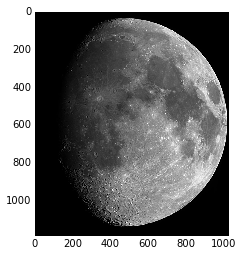
\includegraphics{sample_moon}
\caption{A sample image of the Moon from AstroBin.}
\end{figure}
\subsubsection*{Simple Filtering}
We can take a look at the histogram (Figure 2) of the image to get an idea of the pixel distribution (from 0 to 1) of the grayscale image.
\begin{figure}[h]
\centering
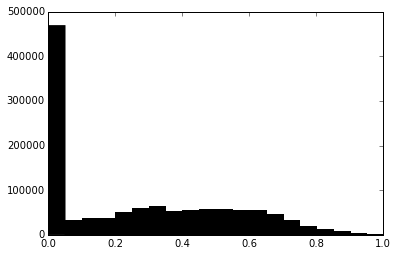
\includegraphics[scale=0.6]{hist}
\caption{Histogram of grayscale pixel values of the sample image. Bin size was increased  to show a broader distribution because of the overwhelming number of 0 values.}
\end{figure}
\pagebreak
\\
Note the peak of low values, which can be attributed to the black background of the night sky of this sample image. By simply filtering the image to select all values above this peak, we get an impressively accurate representation of the current phase of the moon (Figure 3).
\begin{figure}[h]
\centering
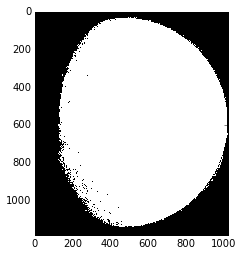
\includegraphics{moon_hist_filtered}
\caption{The sample image filtered by pixels with grayscale value > 0.01.}
\end{figure}
\\
This approach has many limitations. Our sample image conveniently focuses only on the moon and contains a nearly-perfect black background. Other images may contain any number of other objects and may not even contain the moon at all. Indeed, this method only works well in this well-defined case of a cropped image of a moon against a dark background.
\subsubsection*{Otsu's Method}
\subsubsection*{Canny Edge Detection}
\subsubsection*{Region-based Segmentation}
\subsubsection*{Template-matching}
\subsection*{Challenges}
\section*{Future Ideas}
\end{document}